\section{Research Method} \label{sec:research_method}

We adopted Grounded Theory (GT) as the research method. GT is a method
originally proposed by Glaser and Strauss~\cite{glase1967discovery}, which has
as distinguishing features (1) the absence of clear research hypothesis upfront
and (2) limited of literature exposure at the beginning of the research. GT
is a theory-development approach (the hypothesis emerge as the results of
a research investigation), in contrast with more traditional
theory-testing approaches~\cite{coleman2007using}---for instance,  those that
use statistical methods to either confirm or refute pre-established hypothesis.
We used GT as the research method due to the following reasons:

%Some of related work claimed to used ``GT inspired'' approaches\gnote{REF}. It is a very
%common rhetoric in recent research on software engineering, but only research
%that embodies GT’s core principles should claim to be a grounded theory study
%\cite{stol2016grounded}.\gnote{eu removi esse paragrafo pq acho que ele facilmente compraria briga com muitos revisores}

\begin{itemize}

\item GT is a consolidated method in other areas of research - notably medical
sociology \cite{gt_medical_sociology}, nursing \cite{gt_nursing}, education
\cite{gt_education} and management \cite{gt_management}. GT is also being increasingly employed
to study software engineering topics~\cite{hoda2017becoming,stol2016grounded,Waterman:2015:ICSE};

\item GT is considered an adequate approach to investigate scenarios that present
  questions that aims to characterize scenarios under a personal perspective of those
  engaged in a discipline or activite~\cite{barnsteiner2002using},
which is exactly the scenario here: what are the successfull adoption paths for DevOps?

\item GT allows researchers to build an independent and original understanding,
which is adequate to collect empirical evidence directly from the
practice on industry without bias of previous researches. The evidence
is only reintegrated back with the existing literature after the step of
theory construction.

\end{itemize}

Since the publication of the Glaser and Strauss original version of GT~\cite{glase1967discovery},
several modifications and variations have been proposed to the method, coming to
exist at least seven different versions of Grounded Theory~\cite{denzin2007grounded}.
The main versions are those of Glaser, Strauss and
Charmaz~\cite{stol2016grounded}. The study of Stol and colleagues~\cite{stol2016grounded}
explore the main aspects of GT versions and recommend authors of GT studies to
specify which version of the method the study is built upon. Here we chose the classic
Glaser and Strauss version, mainly because we did not have a research
question at the beginning of our research, exactly as suggested in the classic
version. We actually started from an area of interest: successful DevOps adoption
in industry. In addition, research works in software engineering that leverage GT
predominantly use this version~\cite{stol2016grounded}.

% \subsection{GT Procedures}

% In Figure~\ref{fig1}, reproduced from the study of Adolph and colleagues~\cite{adolph2011using}, shows the procedure of the grounded theory research methods followed in the conduction of this
% research.

% \begin{figure}[htpb]
%   \centering
%   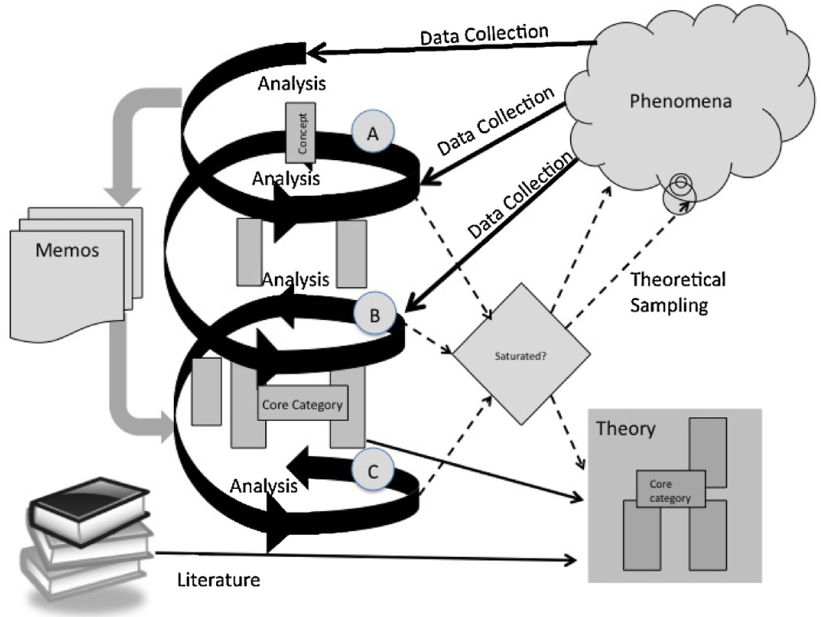
\includegraphics[width=0.5\textwidth,natwidth=821,natheight=617]{GT.png}
%   \caption{The GT Method (reproduced from the study of Adolph and colleagues~\cite{adolph2011using}).}
%   \label{fig1}
% \end{figure}

% This figure depicts four main steps (enumerated as A -- D).

We carried out our research using an existing
guideline about how to conduct a
Grounded Theory~\cite{adolph2011using} research. This guideline organizes
a GT investigation in three steps: \emph{Open Coding} Data Collection,
\emph{Selective Coding} Data Analysis, and \emph{Theoretical Coding}.

%\gnote{acho que antes disso, é preciso dizer como você encontrou e abordou
%os possiveis entrevistados? Jogou um convite nas redes socias? foi por
%conveniencia (p.e., vc conhecia alguem?), etc}
%{\color{red} Welder: Gustavo, eu falei brevemente sobre isso em na subsecao de
%data collection. Voces acham que esses detalhamentos especificos da pesquisa
%deveriam ser unidos com essa parte que explica o metodo de modo mais
%generalista?}

\begin{enumerate}[label=(\Alph*)]
\item {\bf Open Coding Data Collection.} We started our research
  by collecting and analyzing data from companies that have successfully adopted DevOps.
  To this end, we conducted a \emph{raw data analysis} that search for patterns of
  incidents to indicate concepts,  and then grouped these concepts into
  categories~\cite{stol2016grounded}.

\item {\bf Selective Coding Data Analysis.} In the second step we evolve
  the initial set of
  categories by comparing new incidents with the previous ones. Here the goal is
  to identify a ``core category''~\cite{stol2016grounded}.
  The core category is responsible for enabling the integration of the other
  categories and structuring the results into a dense and consolidated grounded
  theory~\cite{jantunen2014using}. The identification of the core category
  represents the end of the open-coding phase and the beginning of the selective coding.
  In the selective coding, we only consider the specific variables that are directly
  related to the core category, in order to enable the production of an harmonic
  theory~\cite{coleman2007using,hoda2011impact}. Selective coding ends when we
  achieve a theoretical saturation, which occurs when the last few
  participants provided more evidence and examples but no new concepts or
  categories~\cite{glase1967discovery}.

\item {\bf Theoretical Coding.} After saturation, we built a theory that
explains the categories and the relationships between the categories.
Additionally, we reintegrated our theory with the existing literature, {\color{red}which allowed us to compare our proposal
 with other theories about DevOps}. That is, using a Grounded Theory approach,
 one should only conduct a literature review in later stages of a research,
in order to avoid external influences to conceive a theory~\cite{adolph2012reconciling}.

\end{enumerate}

Throughout the process, we wrote memos capturing thoughts and analytic
processes; the memos support the emerging concepts, categories, and their
relationships~\cite{adolph2012reconciling}.

%\gnote{para cada um dos itens acima, poderiamos colocar exemplos reais
%do trabalho? p.e., citar 1-2 memos?}
% Welder: inseri um exemplo de coding na sequencia do artigo.

% The following sub-sections present details of procedures applied in this study,
% containing some examples to illustrate their application.

% \subsection{Data Collection}

Regarding data collection, we conducted semi-structured interviews with 15 practitioners of companies from
Brazil, Ireland, Portugal, Spain, and United States. These practitioners
contributed to DevOps adoption processes in their companies. Participants
were recruited using two approaches: (1) through direct contact in a \emph{DevOpsDays}
event in Brazil and (2) through  general
calls for participation posted on DevOps user groups, social networking sites,
and local communities. In order to achieve a heterogeneous perspective
and increase the potential of generalization of the results,
we consulted practitioners from a variety of companies.
Table~\ref{participant_table} presents the characteristics of the participants
that accepted our invitation.
To maintain anonymity, in conformance with the human ethics guidelines,
hereafter we will refer to the participant as P1--P15 (first column).
%The second column shows the role of
%each participant in her respective company. The remaining columns list their
%software development experience in years (SX), DevOps experience in years (DX),
%country of work (CN), main domain of the company, and company size (CS).


\begin{table}[t]
\centering
\caption{Participant Profile. SX means software development experience in years,
DX means DevOps experience in years, CN means country of work, and CS means
company size (S<100; M<1000; L<5000; XL>5000)).}
\label{participant_table}
\begin{tabular}{|p{0.4cm}|p{2.6cm}|p{0.4cm}|p{0.45cm}|p{0.5cm}|p{1.3cm}|p{0.3cm}|} \toprule \centering
\textbf{P\#}          & \textbf{Role}
       & \textbf{SX} & \textbf{DX} & \textbf{CN}   & \textbf{Domain}    & \multicolumn{1}{l}{\textbf{CS}} \\ \midrule \centering
P1                   & DevOps Developer      & 9            & 2           & IR            & IT                 & S                               \\ \centering

P2                   & DevOps Consult.       & 9            & 3           & BR            & IT                 & M                               \\ \centering

P3                   & DevOps Developer      & 8            & 1           & IR            & IT                 & S                               \\ \centering

P4                   & Computer Tech.        & 10           & 2           & BR            & Health             & S                               \\ \centering

P5                   & Systems Engineer      & 10           & 3           & SP            & Telecom            & XL                              \\ \centering

P6                   & Developer             & 3            & 1           & PO            & IT                 & S                               \\ \centering

P7                   & Support Analyst       & 15           & 2           & BR            & Telecom            & L                               \\ \centering

P8                   & DevOps Engineer       & 20           & 9           & BR            & Marketing              & M                               \\ \centering

P9                   & IT Manager            & 14           & 8           & BR            & IT                 & M                               \\ \centering

P10                  & Network Admin.        & 15           & 3           & BR            & IT                 & S                               \\ \centering

P11                  & DevOps Superv.                & 6            & 4           & BR            & IT                  & M                               \\ \centering

P12                  & Cloud Engineer              & 9            & 3           & US            & IT                  & L                               \\ \centering

P13                  & Technology Mngr.                 & 18            & 6           & BR            & Food                  & M                               \\ \centering

P14                  & IT Manager            & 7            & 2           & BR            & IT                  & S                               \\ \centering

P15                  & Developer        & 3            & 2           & BR            & IT                  & S \\ \bottomrule
\end{tabular}
\end{table}



The interview were conducted over one year using Skype calls.
Data collection and analysis were iterative so the collected data of a given interview helped guide
future interviews. The questions of interview evolved according to
the progress of the research. We start with five open-ended questions: (1) What
motivated the adoption of DevOps? (2) What adopt DevOps means in the context of
your company? (3) How was DevOps adopted in your company? (4) What were the
results of adopting DevOps? And (5) What were the main difficulties?

As the analyzes were being carried out, new questions were added to the script.
These new questions were related to the concepts and categories identified in
previous interviews. Examples of new questions include: (1) What is the
relationship between deployment automation and DevOps adoption? (2) Is it
possible to adopt DevOps without automation? (3) How does your company fostered a collaboration
culture?

With respect to \emph{data analysis}, the interviews were voice recorded, transcribed, and analyzed. The first moment
of the analysis, called open coding in GT, started immediately after the
transcription of the first interview, which
was used to evolve the interview script to be used in
the second interview, and so on. The open coding lasted until there was no
doubt about the core category of the study. Similar to what is described in
the work of Adolph and colleagues~\cite{adolph2012reconciling}, we started
with a strong candidate core category yet not consolidated. Until
the analysis of the fourth interview, we cogitated \emph{automation} as core
category because it is a recurring pattern in our data. However, we quickly
realized that the ``automation" category did not explain most of the behaviors
or events in our data. At the same time, we started to understand that
\emph{collaboration culture} also appeared recurrently in the analysis and with more
potential to explain the remaining events. We then started to ask explicitly
about the role of the automation and how the collaboration culture is formed
in a DevOps adoption process.

After the adaptations made in the script and analysis of new data in a constant
comparison process, taking into account the previous analyses and the
respective memos written during all the process, after the analysis of the tenth
interview, we concluded that ``collaboration culture" was unequivocally the core
category regarding how DevOps was successfully adopted in the studied companies.
At this moment, the open coded ended and the selective coding started.

After the discovery of the core category, we started to restrict the coding only
to specific variables that were directly related to the core category and their
relationships: the selective coding.
With more three interviews and respective analysis, we realized that
the new data added less and less content to the emerging theory. That is, the
explanation around how the collaboration culture is developed providing
DevOps adoption showed signs of saturation. We then conducted more two
interviews to conclude that we had reached the theoretical saturation.

After saturation, we started the theoretical coding to find a way to integrate
all the concepts, categories and memos in the form of a cohesive and
homogeneous theory, where we have pointed out the role of the categories as
enablers and outcomes, as shown above. We present more details about
the results of our theoretical coding phase in the next section.

To illustrate the coding procedures, we present an example of working from
interview transcript to category.

Raw interview transcripts are full of noise. So we start the coding by removing
this noise, identifying the key points. Key points are the summarized points
from sections of the interview~\cite{georgieva2008best}. Example:

\textbf{Raw data:} \textit{``So, here we adopted this type of strategy that is
the infrastructure as code, consequently we have the versioning of our entire
infrastructure in a common language, in such a way that any person, a
developer, an architect, the operations guy of even the manager, he looks and
is able to describe that the configuration of application x is y. So, it
aggregates too much value for us exactly with more transparency"}

\textbf{Key point:} \textit{``Infrastructure as code contributes to
transparency because it enables the infrastructure versioning in a common
language to all professionals"}

We then assigned a code to the key point. A code is a phrase that summarizes
the key point and one key point can lead to several codes
\cite{hoda2017becoming}.

\textbf{Code:} \textit{Infrastructure as code contributes to transparency}

\textbf{Code:} \textit{Infrastructure as code provides a common language}

In this example, the concept that emerged was ``infrastructure as code". The
expression corresponding to this concept comes directly from raw data, but this
is not a rule. It is common for the concept to be an abstraction, without
emerging from an expression present in raw data.

At this moment in the analysis, we already had identified another concepts that
contribute to transparency. We wrote the following memo:

\textbf{Memo:} \textit{Similar to sharing on a regular basis and shared
pipelines, the concept of infrastructure as code is related as important to
transparency. These transparency related concepts have often been cited as
means to achieve greater collaboration between teams}.

The constant comparison method was repeated on the concepts to produce a third
level of abstraction called categories. The concepts sharing on regular basis,
shared pipelines and infrastructure as code were grouped into
\textbf{transparency} category.

%\gnote{seria bom linkar aqui os itens A--B descritos na seção anterior.}
